%!TEX root = main.tex
\section{Background}
\label{sec:background}
% \subsection{Deep Learning Parallel Training}
% The deep neural network (DNN) can be defined as a sequence of layers,
% where each layer is composed of a forward computation function and its associated parameters.
% Due to the increasingly scale of modern DNNs and the size of training dataset,
% training new DNN models on single GPU is becoming more and more impossible.
% Thus, training DNNs in parallel on multiple GPUs or nodes becomes more and more significant.
% % Thus, several parallel approaches have been proposed to train the model in parallel.

% Typically, there are mainly three kinds of parallel approaches,
% including \emph{Data Parallelism}, \emph{Tensor Parallelism}, and \emph{Pipeline Parallelism}.
% Data parallelism (DP) is the most widely used parallel strategy which
% divides the training data into multiple shards and distribute them to different devices.
% Each device stores a full replica of the model parameters.
% At each step, it begins by leveraging its local data for forward propagation,
% subsequently engaging in communication with other devices to synchronize
% and update the global model parameters at backward propagation.
% The disadvantages of data parallelism are obvious especially when the model is increasingly large.
% Firstly, it suffers from memory pressure since each device needs to hold a full replica of model parameters.
% Secondly, the communication overhead is very large as each device needs to
% send its own updated model to synchronize and integrate with each other.
% ZeRO~\cite{rajbhandariZeROMemoryOptimizations2020} optimizes the memory efficiency
% of data parallelism via eliminating the model's parameters redundancy across devices.
% It is achieved by distributing the model states evenly across the devices.
% The model states include parameters,
% gradients, and optimizer states (such as the moving averages in the Adam optimizer).
% It uses \emph{pull/push} communication operations when the model states is holded by other devices.

% Tensor Parallelism (TP) which can also be named as intra-operator parallelism,
% targets the inherent parallel structure of DNNs.
% In this parallelism paradigm, computations are parallelized across the dimensions of tensors,
% the fundamental data structures in DNNs.
% It splits a tensor into $N$ chunks ($N$ devices) along a particular dimension
% such that each device holds $\frac{1}{N}$ of the whole tensor.
% Each device perform the computation on its tensor chunk to get the partial result.
% These partial result will be collected from each device and integrated into the full output.
% The next layer's computation can only start until the previous layer's communication completes.
% Therefore, the communication in TP cannot be overlapped with the computation,
% which means a very high inter-device communication bandwidth is demanded
% to reduce the communication overhead for TP.
% Megatron-LM~\cite{shoeybi2019megatron} proposed by NVIDIA is a famous research work which manually
% partitions the large language model in the tensor parallel manner.
% In the meanwhile,
% due to the fact that each layer's input/output can be split at various dimension,
% the total parallel solution search space is a huge when considering the whole model's tensor parallelism.
% By that, there are lots of automatic tensor parallelism search and code generated works in both academia and industry.

% Pipeline Parallelism (PP) aims to parallelize the computation between layers which
% partitions the DNNs to several layers chunk and dispatches them to different stages (devices).
% Meanwhile, it also divides the input data of an iteration (a minibatch) into several micro-batches,
% which can be processed in parallel by the pipeline stages.
% Once a stage completes the forward pass for a micro-batch,
% the activation memory is communicated to the next stage in the pipeline.
% Similarly, as the next stage completes its backward pass on a micro-batch,
% the gradient with respect to the activation is communicated backwards through the pipeline.
% It's obvious that the communication of activation/gradient memory can be overlapped with the computaiton.
% Due to the fact that the activation/gradient memory size is usually smaller than the whole model's parameters,
% the communication overhead of pipeline parallelism is the smallest
% across these three parallel paradigm in general, which can be reduced by up to 95\%~\cite{narayanan2019pipedream}.
% By breaking down the DNNs into stages and overlapping the execution of these stages, 
% pipeline parallelism minimizes idle time and maximizes hardware utilization, thus accelerating the training process.

\subsection{Synchronous and Asynchronous Pipeline Parallelism}
Pipeline parallelism aims to parallelize the computations between
different layers of a neural network by dividing the model into
multiple layer blocks and assigning them to different stages (GPUs).
It divides the input of a batch
into multiple micro-batches, enabling pipeline parallel execution among different stages.
Once a stage completes the forward computation of a micro-batch,
the activation memory is transferred to the next stage.
Similarly, when the last stage completes the forward computation
and loss calculation of a micro-batch,
the gradients computed by the backward computation are conveyed 
in the reverse direction of the pipeline until they reach the first stage.
% It is evident that in pipeline parallelism, the communication of
% activation and gradient memory can overlap with computation,
% and since the size of activation values and gradient memory
% is usually smaller than the parameters of the entire model
% and is only transferred between adjacent stages,
% the communication overhead of pipeline parallelism is
% typically the smallest among the three parallel methods, potentially reducing it by up to 95%[13].

According to the different ways of updating model parameters,
the pipeline parallelism can be divided into two categories:
\emph{Synchronous Pipeline Parallelism (SPP)} and \emph{Asynchronous Pipeline Parallelism (ASP)}.
The SPP performs the same as the synchronous
parameters update in single GPU training.
This means the next mini-batch's computation won't start until
the preceding mini-batch's backward propagation finished updating the model parameters.
GPipe~\cite{huangGpipeEfficientTraining2019} proposed by Huang et al.
is the most representative SPP work,
whose execution manner is shown as Figure~\ref{fig:gpipe}.
Each small rectangle in the figure represents the forward (color)
and backward (color) computation on a micro-batch
and the number in the rectangle represents the micro-batchs' number.
There are total four GPUs and the same number of the micro-batches are fed into the pipeline.
It's obvious that the SPP cannot achieve high GPU utilization
since there is a synchronization barrier before the next mini-batch's pipeline execution.
This will introduce the pipeline bubbles (idle GPU time)
which are shown as the blank area in Figure~\ref{fig:gpipe}.

% and DAPPLE~\cite{fan2021dapple}
To solve the low GPU utilization problem in SPP,
PipeDream~\cite{narayananPipeDreamGeneralizedPipeline2019} proposes an ASP method
which adopts a 1F1B scheduling mechanism to improve the GPU utilization.
Its execution manner is shown as Figure~\ref{fig:pipedream}.
It has a warm-up phase to initialize the pipeline.
Specifically, the $(n-x)$ number of micro-batches in $x$ stage need to be fed into the pipeline
in order to perform the 1F1B scheduling.
In order to guarantee the parameter consistency in the same micro-batch's forward and backward
multiple parameters versions need to be maintained in this parallelism paradigm.
Specifically, the $(n-x)$ replicas of parameters need to be maintained for the stage of $x$,
i.e., the former stage needs more GPU memory to stores the parameters replicas.
DAPPLE~\cite{fanDAPPLEPipelinedData2021} introduce the 1F1B computation scheduling to GPipe
to optimize the computation efficiency of synchronous PP.
% Dapple need to set the number of the micro-batches to be at least double of the number of stages in order to perform 1F1B scheduling
% TODO(hp): do we need to define notations first
In recent years, there are lots of works~\cite{sunAdaPipeOptimizingPipeline2024,vzhaoVPipeVirtualizedAcceleration2022,liChimeraEfficientlyTraining2021,kimBPipeMemoryBalancedPipeline2023}
to optimize the efficiency of PP,
they all follow either GPipe or PipeDream's computation scheduling as the basis.
% \begin{figure}
%   \centering
%   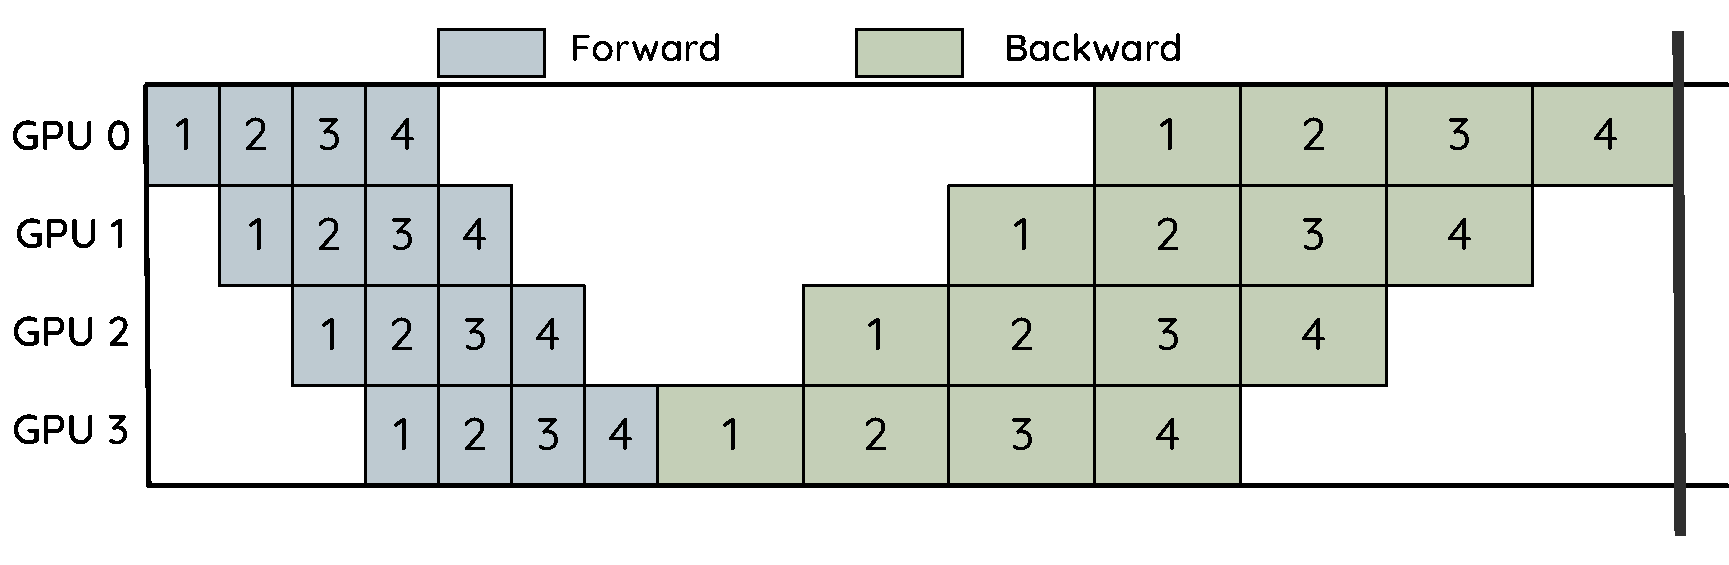
\includegraphics[width=0.95\linewidth]{GPipe-execution.pdf}
%   \caption{GPipe's Synchronous Pipeline Parallelism}
%   \label{fig:gpipe}
% \end{figure}
% \begin{figure}
%   \centering
%   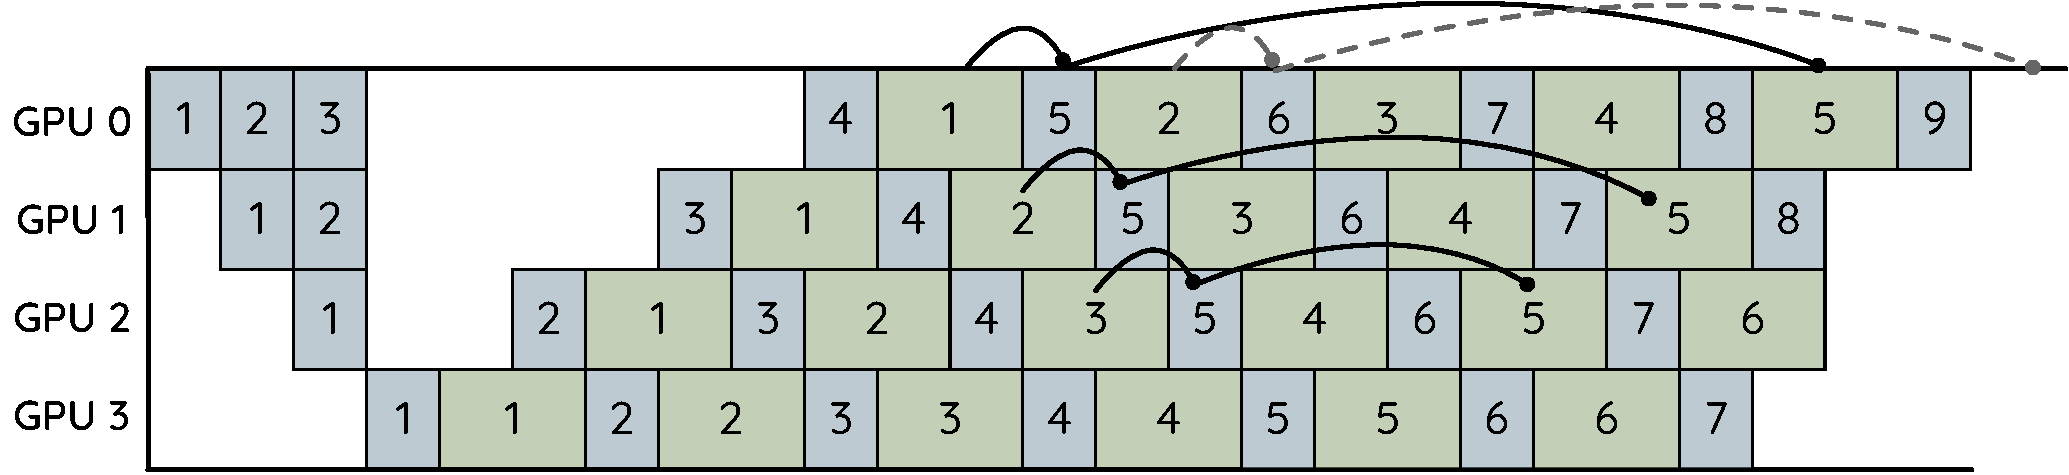
\includegraphics[width=0.95\linewidth]{PipeDream-execution.pdf}
%   \caption{PipeDream's Asynchronous Pipeline Parallelism}
%   \label{fig:pipedream}
% \end{figure}
\begin{figure}[htb]
  \centering
  % \hspace{-0.7cm}
  \subfigure[Synchornous Pipeline Parallel — GPipe]{
    \centering
    \label{subfig:gpipe}
    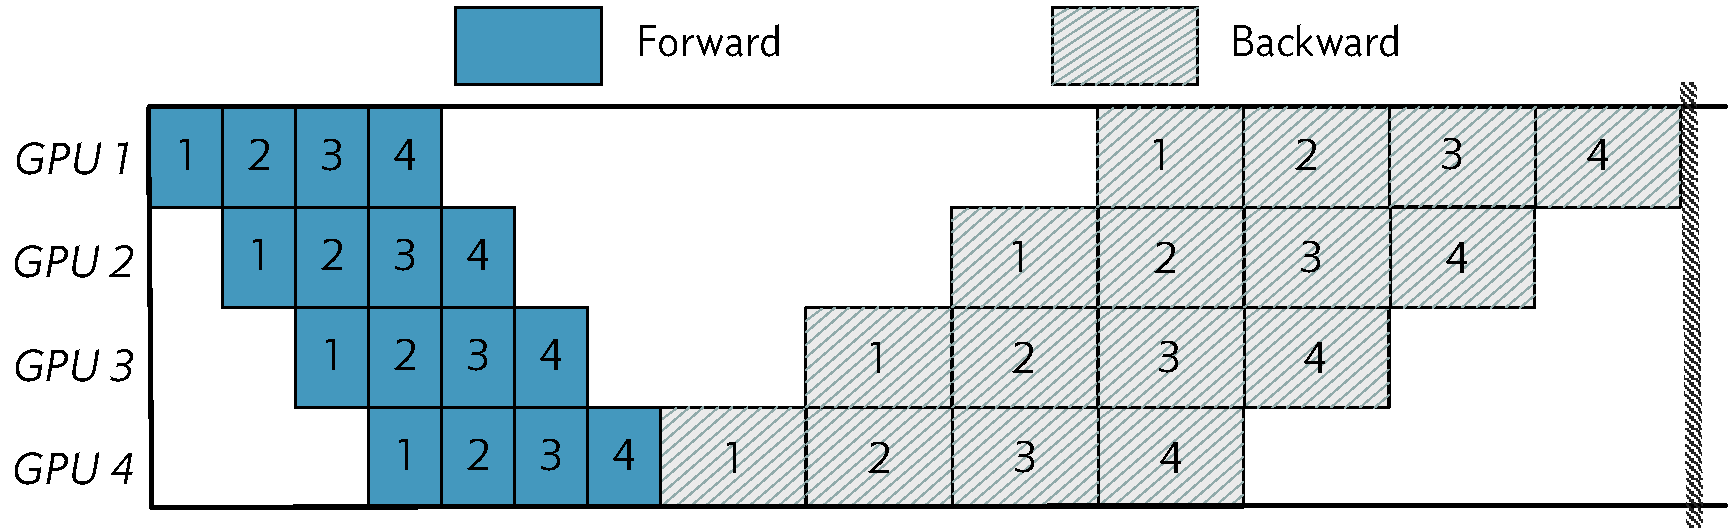
\includegraphics[width=1.0\linewidth]{GPipe-exec.pdf}
  }
  \subfigure[Asynchronous Pipeline Parallel — PipeDream]{
    \centering
    \label{subfig:pipedream}
    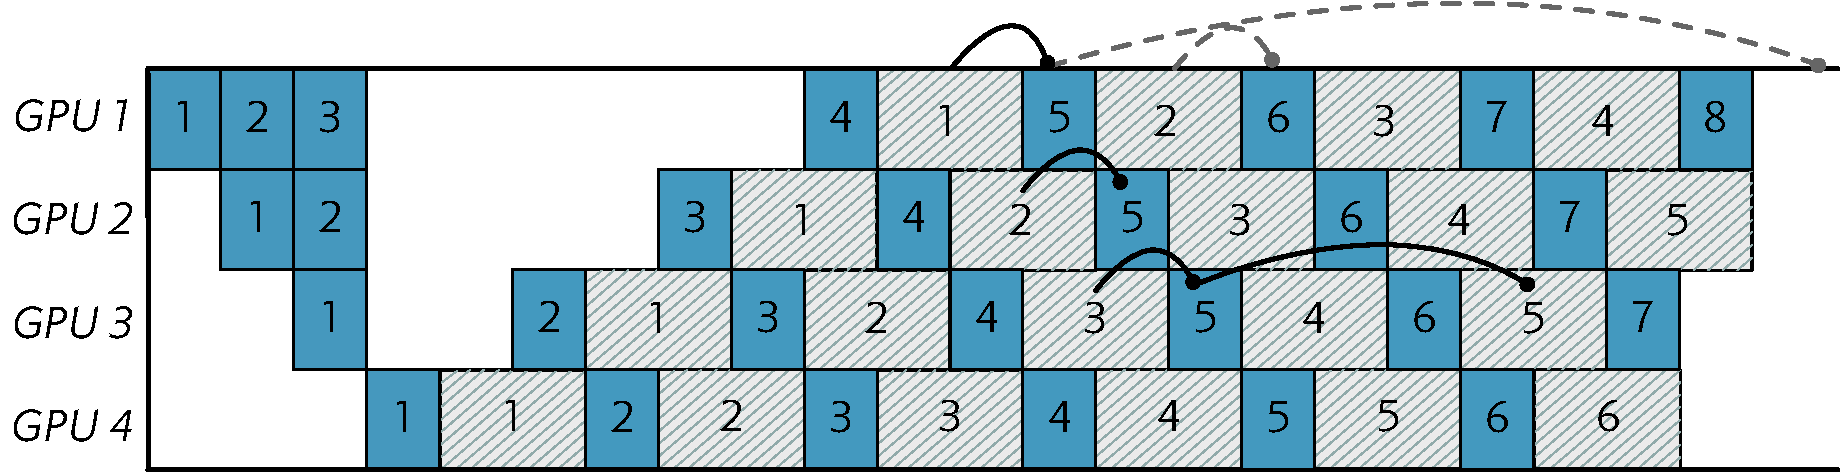
\includegraphics[width=1.0\linewidth]{PipeDream-exec.pdf}
  }
  \caption{Synchornous and Asynchronous Pipeline Parallel Execution}
  \label{fig:pp-exec}
\end{figure}

\subsection{Swap and Recomputation}
In previous works~\cite{vrhuVDNNVirtualizedDeep2016,chenTrainingDeepNets2016,wangSuperneuronsDynamicGPU2018,pengCapuchinTensorbasedGPU2020}
of memory optimization for DL training,
swap and recomputation (also named as \emph{activation checkpointing})
are already been proved to be two
effective approaches to reduce the memory footprint during the DNN's training.
Both \emph{swap} and \emph{recomputation} utilize the characteristic that
there is a time gap between two accesses to the same activation memory
in forward and backward propagation.
Swap aims to leverage the CPU memory as the external memory to extend the GPU memory limitation.
which copies the activation memory to CPU in forward pass
and copy back to GPU in backward pass, in which the vDNN~\cite{rhuVDNNVirtualizedDeep2016} is the pioneer.
Chen et al.~\cite{chenTrainingDeepNets2016} proposed the activation checkpointing technique to drop the
activation memory during forward propagation and perform the forward computation
again to regenerate the activation memory, which will incur about 30\% overhead to the overall training.
SuperNeurons~\cite{wangSuperneuronsDynamicGPU2018} and Capuchin~\cite{pengCapuchinTensorbasedGPU2020} proposes dynamic
swap and recomputation strategies to further reduce the memory footprint while maintaining training performance.
Wahib et al.~\cite{wahib2020scaling} added the swap memory optimization support in distributed training environment.
% TODO(hp): add related works for distributed environment
For pipeline parallelism,
GPipe~\cite{huangGpipeEfficientTraining2019} has integrated the recomputation mechanism.
vPipe~\cite{zhaoVPipeVirtualizedAcceleration2022} further propose a iterative pipeline partition algorithm
that considers \emph{swap, recomputation}, and \emph{partition} in conjunction.
AdaPipe~\cite{sunAdaPipeOptimizingPipeline2024} proposed a two-step dynamic programming algorithm
of pipeline partitioning and re-computation strategy for the 1F1B computation scheduling.
% However, these works perform model partitioning and memory optimization
% are all at a coarse granularity (layer block), which make it difficult to
% achieve both the memory and computation efficiency.
% Besides, they ignores the computation characteristics differences
% between the pipeline parallelism and single-GPU training,
% which cannot support efficient memory swap in pipeline parallelism.

% In recent years, the scale of deep neural networks has been growing increasingly large,
% especially in the field of natural language processing,
% such as large models like T5, GPT-4, and Huawei's PanGu.
% The memory capacity of a single GPU is no longer sufficient to accommodate such large-scale models,
% making the use of multiple GPUs for parallel training a common choice in both academia and industry.
% Among these parallel methods, data parallelism requires all GPUs to synchronize and update the entire
% model parameters in each iteration. As the model parameters grow larger, this communication overhead
% becomes increasingly significant. Tensor parallelism not only requires careful division of model operators
% but also necessitates synchronous communication between divided operators, which affects computational performance.
% Pipeline parallelism, in contrast to the two methods mentioned above, usually has much less communication volume
% because communication only occurs between adjacent stage GPUs, with the amount of communication being
% only the activation values and gradients at the division points.
% Moreover, this communication can be executed in parallel with computation,
% thus attracting extensive research and attention in the industry.
% However, due to the constraints of model division,
% pipeline parallelism often leads to a significant waste of GPU memory resources to ensure overall training performance,
% limiting the scale of the models it can support.
